\chapter{Superconduttori}
La superconduttività venne scoperta nel 1911 da Kamerlingh Onnes raffreddando del mercurio tramite l'elio liquido. Si osservò che la conduttività del mercurio aumentava al diminuire della temperatura, quindi la resistenza diminuiva per via della diminuizione degli urti degli elettroni. Però al di sotto di una certa temperatura detta \textbf{temperatura critica} la resistenza R va a zero. Quindi inizialmente si disse che il mercurio era passato ad un nuovo stato nel quale esibiva straordinarie proprieta conduttive chiamato stato superconduttivo.
\section{Effetto Meissner e Variabile di Stato}
Ciò che distingue un semplice conduttore con resistenza molto bassa da un vero superconduttore è la presenza dell'\textbf{effetto Meissner}. Questo fenomeno consiste nell'espulsione totale del campo magnetico dal volume del materiale non appena esso entra nello stato superconduttivo. In altre parole, un superconduttore non permette la penetrazione del campo magnetico interno, indipendentemente dalle condizioni esterne precedenti.
\subsection*{Ragionamento Fisico-Matematico}
Consideriamo il seguente ragionamento: se la resistenza di un materiale tende a zero, allora la conduttività \(\sigma\) tende all'infinito. Dato che la legge di Ohm locale è espressa da
\[
J = \sigma E,
\]
per mantenere una densità di corrente \(J\) finita con \(\sigma \to \infty\) è necessario che il campo elettrico \(E\) sia nullo (altrimenti \(J\) diverrebbe infinito). 
Utilizzando ora la legge di Faraday,
\[
\vec{\nabla} \times E = -\frac{1}{c}\,\frac{\partial B}{\partial t},
\]
se \(E = 0\) allora la sua rotazione è nulla, il che implica che:
\[
\frac{\partial B}{\partial t} = 0.
\]
Questa condizione significa che, se fosse presente un campo magnetico \(B\) all'interno del materiale, esso non cambierebbe nel tempo. Un'analisi superficiale porterebbe dunque a ipotizzare che, al passaggio nello stato superconduttivo, il campo magnetico interno resti costante.
\subsection*{Il Paradosso e l'Effetto Meissner}
Nonostante il ragionamento precedente, le osservazioni sperimentali mostrano che, al calar della temperatura al di sotto di una soglia critica \(T_c\), il materiale espelle il campo magnetico, ottenendo un campo interno nullo (\(B = 0\)). Questo è l'\textbf{effetto Meissner}.\\\\
L'espulsione del campo magnetico fa sì che il campo magnetico non sia una quantità “congelata” (dipendente dalla storia del campione) ma diventi una vera e propria \textbf{variabile di stato}. Ciò significa che lo stato finale di un superconduttore (con \(B = 0\)) è univocamente determinato dalle sue condizioni termodinamiche, indipendentemente dal percorso seguito per raggiungerlo.
\subsection*{Verifica tramite Esperimenti con Sequenze Differenti}
Per mettere in evidenza questo aspetto, consideriamo due procedure sperimentali che portano al medesimo stato finale:
\begin{enumerate}
    \item \textbf{Sequenza con Effetto Meissner:}\\
    In un primo esperimento (vedi Figura \ref{fig:eff}), il materiale viene inizialmente tenuto nello stato normale (temperatura \(T > T_c\)) in presenza di un campo magnetico \(B \neq 0\). Successivamente, raffreddando il materiale al di sotto della temperatura critica, si osserva che il campo magnetico viene espulso, ottenendo infine uno stato superconduttivo in cui \(B = 0\).

    \item \textbf{Sequenza con Raffreddamento Diretto:}\\
    In un secondo esperimento (vedi Figura \ref{fig:eff} a sinistra), il materiale viene prima raffreddato direttamente a \(T < T_c\) e, solo a valle, viene applicato un campo magnetico. In questo caso, il campo non riesce a penetrare nel materiale già superconduttivo, e si ottiene nuovamente un superconduttore con \(B = 0\).
\end{enumerate}
Questi due itinerari portano sempre allo stesso stato finale, dimostrando che il campo magnetico all'interno del superconduttore è una variabile di stato. \\
Al contrario, in assenza dell'effetto Meissner (vedi Figura \ref{fig:noeff}), se il campo magnetico fosse "congelato" nello stato in cui il materiale entra nel regime superconduttivo, la storia del campione determinerebbe lo stato interno. Ad esempio:
\begin{itemize}
    \item Nel primo caso, il materiale, raffreddato in presenza di \(B\), mantenendolo costante a causa di \(\frac{\partial B}{\partial t}=0\), presenterebbe un campo magnetico interno non nullo.
    \item Nel secondo caso, il materiale raffreddato in assenza di campo resterebbe con \(B = 0\).
\end{itemize}
Le due situazioni darebbero così esiti differenti, contraddicendo il concetto di variabile di stato. 

\begin{figure} [H]
    \centering
    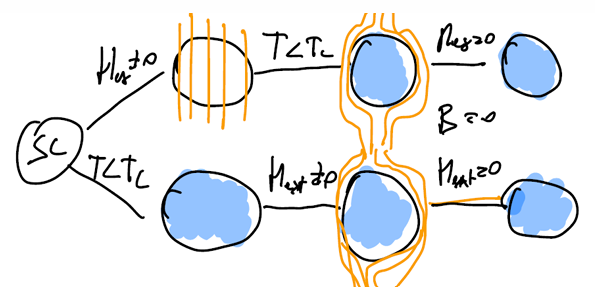
\includegraphics[width=0.7\linewidth]{images/10-Superconduttori/eff meissner.png}
    \caption{}
    \label{fig:eff}
\end{figure}
\begin{figure} [H]
    \centering
    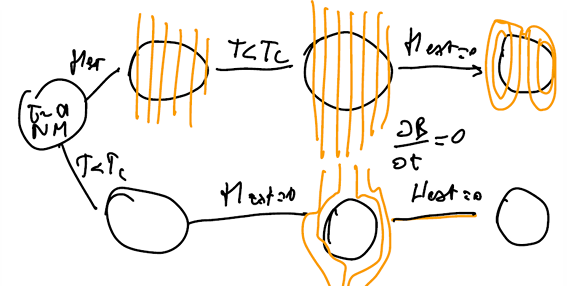
\includegraphics[width=0.7\linewidth]{images/10-Superconduttori/no eff meissner.png}
    \caption{}
    \label{fig:noeff}
\end{figure} 

\section{Origine del Passaggio di Stato e Effetto Meissner}

Il passaggio di stato che porta un materiale a diventare superconduttore non è accompagnato da alcuna modifica della struttura cristallina. Infatti, se si irragge il campione con raggi-X si osserva che la disposizione degli atomi non cambia, e non si registrano transizioni che coinvolgono l'ordine magnetico (ad es. transizioni ferromagnetiche o antiferromagnetiche). \textbf{La transizione è invece dovuta a un cambiamento nello stato elettronico: al passaggio alla fase superconduttiva si apre un gap nell'energia dei livelli elettronici in prossimità del livello di Fermi. Tale apertura comporta una modifica della densità degli stati disponibili e, conseguentemente, delle quantità termodinamiche come l'energia libera e il calore specifico.}

\subsection*{Effetti sul Calore Specifico e sull'Energia Libera}

Osservando l'andamento del calore specifico \(C_V\) e dell'energia libera \(F\) (vedi Figura \ref{fig:calspF}), si evidenzia come la presenza del gap influisca notevolmente sulle proprietà termodinamiche:
\begin{itemize}
    \item \textbf{Calore Specifico:} Nel metallo normale la distribuzione degli stati elettronici attorno al livello di Fermi è continua. Con l'apertura del gap, il numero di stati a disposizione in prossimità di \(E_F\) diminuisce, modificando il contributo entropico del sistema. Questo si traduce in un andamento del calore specifico che differisce sensibilmente da quello del metallo normale.
    \item \textbf{Energia Libera:} La variazione dell'energia libera tra lo stato normale (\(F_N\)) e quello superconduttivo (\(F_S\)) è legata all'energia necessaria per espellere il campo magnetico dal materiale, secondo il rapporto:
    \[
    F_N(T) - F_S(T) = \frac{H_C(T)^2}{8\pi}.
    \]
    Tale termine rappresenta l'energia di espulsione del campo magnetico e risulta strettamente connesso alla variazione dell'entropia tra i due stati.

    \begin{figure}[H]
        \centering
        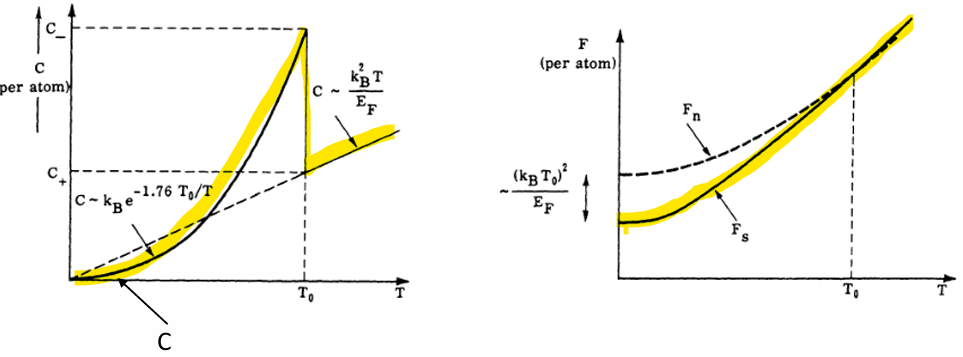
\includegraphics[width=0.9\linewidth]{images/10-Superconduttori/calspF.png}
        \caption{La linea tratteggiata rappresenta l'andamento termodinamico del metallo normale, mentre quella continua evidenzia l'andamento del superconduttore.}
        \label{fig:calspF}
    \end{figure}
\end{itemize}

\subsection*{Superconduttori di Tipo I}
I superconduttori si distinguono in due classi in base alla loro risposta al campo magnetico: \textbf{Tipo I} e \textbf{Tipo II}. Nei superconduttori di Tipo I il campo magnetico viene completamente espulso (effetto Meissner). \\
Considerando il campo magnetico applicato \(H\) come variabile di stato, si può ricavare un diagramma di fase in funzione della temperatura (vedi Figura \ref{fig:diagfaseH1}):
\begin{figure}[H]
    \centering
    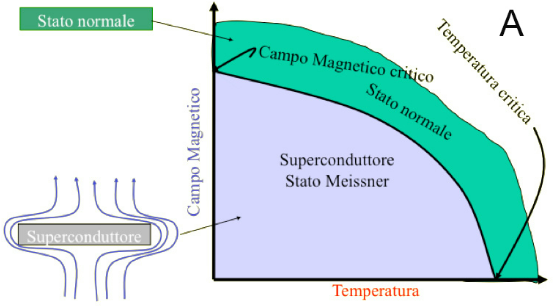
\includegraphics[width=0.7\linewidth]{images/10-Superconduttori/diagfaseH.png}
    \caption{Diagramma di fase per un superconduttore di Tipo I.}
    \label{fig:diagfaseH1}
\end{figure}

Dal diagramma risulta che:
\begin{itemize}
    \item Quando \(H > H_c(T)\) il materiale resta nello stato normale.
    \item Quando \(H < H_c(T)\) il materiale entra nello stato superconduttivo, espellendo il campo magnetico mediante la generazione di correnti di schermo sulla superficie.
\end{itemize}

Il fatto che il superconduttore impieghi una certa quantità di energia per espellere il campo magnetico è correlato alle variazioni entropiche. Per analizzare questo punto si consideri l'energia libera di Helmholtz. Al punto di transizione, quando lo stato normale e quello superconduttivo coesistono, si ha:
\[
F_N(T) = F_S(T) + \frac{H_C(T)^2}{8\pi},
\]
da cui
\[
F_N(T) - F_S(T) = \frac{H_C(T)^2}{8\pi}.
\]
Derivando questa relazione rispetto a \(T\), si ottiene:
\[
\frac{d}{dT}\Bigl[ F_N(T)-F_S(T) \Bigr] = \frac{H_C(T)}{4\pi}\frac{dH_C(T)}{dT}.
\]
Ricordando che l'entropia \(S\) è definita da \(S = -\frac{\partial F}{\partial T}\), segue:
\[
S_S - S_N = \frac{H_C(T)}{4\pi}\frac{dH_C(T)}{dT}.
\]
Dal diagramma di fase, si osserva che \(\frac{dH_C(T)}{dT} < 0\). Quindi:
\[
S_S < S_N,
\]
ovvero la transizione al regime superconduttivo è accompagnata da una diminuzione dell'entropia.

\subsection*{Espulsione del Campo Magnetico e Gap Elettronico}
\textbf{L'espulsione completa del campo magnetico nei superconduttori di Tipo I si ottiene mediante la formazione di correnti di schermo che scorrono in prossimità della superficie del materiale.} Queste correnti creano un campo magnetico che, per effetto di interferenza, annulla il campo esterno all'interno del superconduttore.\\\\

Un ulteriore aspetto fondamentale riguarda il meccanismo che porta alla formazione del gap a livello dell'energia di Fermi. Si può osservare questo fenomeno tracciando la funzione
\[
f\ln f - (1-f)\ln (1-f),
\]
dove \(f\) è la distribuzione di Fermi-Dirac, in funzione del rapporto \(E/E_F\) (vedi Figura \ref{fig:eef}). Tale funzione risulta fortemente concentrata in prossimità di \(E_F\). \\
\textbf{Per ridurre l'entropia e ottenere così un minor numero di stati accessibili nei dintorni di \(E_F\), il sistema evolve in modo da aprire un gap nell'energia dei livelli elettronici.} La riduzione degli stati disponibili è direttamente responsabile della diminuzione dell'entropia che abbiamo osservato derivando l'energia libera.
\begin{figure}[H]
    \centering
    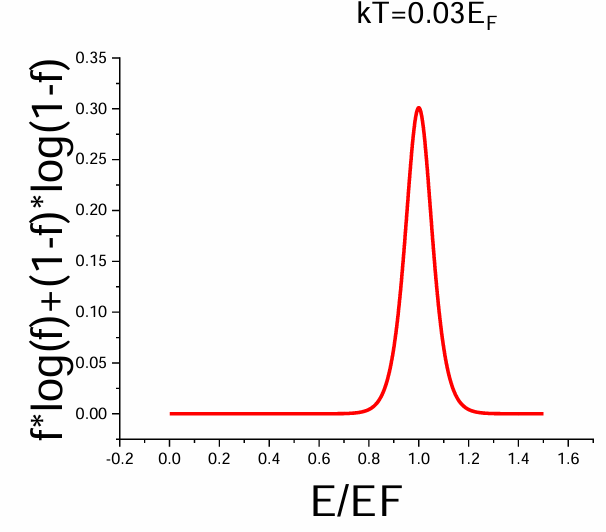
\includegraphics[width=0.7\linewidth]{images/10-Superconduttori/eef.png}
    \caption{Comportamento della funzione \(f\ln f - (1-f)\ln (1-f)\) in funzione di \(E/E_F\). La forte concentrazione in prossimità di \(E_F\) evidenzia come un gap riduca il contributo entropico degli elettroni.}
    \label{fig:eef}
\end{figure}

\subsection*{Calcolo del Calore Specifico al Punto di Transizione}
Per esaminare il punto di transizione, si studia il salto nel calore specifico, che è direttamente collegato alla variazione dell'entropia. Partiamo dalla relazione:
\[
\Delta S = \frac{H_C(T)}{4\pi} \frac{dH_C(T)}{dT}.
\]
Il calore specifico a volume costante in prossimità della temperatura critica \(T_C\) è definito come:
\[
c_V(T_C) = T_C \left( \frac{\partial S}{\partial T} \right)_V.
\]
Calcolando la derivata dell'entropia rispetto a \(T\) si ottiene:
\[
c_V(T_C) = \frac{T_C}{4\pi} \left[ \left( \frac{dH_C}{dT} \right)^2 + H_C(T_C) \left( \frac{d^2 H_C}{dT^2} \right) \right].
\]
Poiché per definizione \(H_C(T_C)=0\) (al punto di transizione il campo critico si annulla), il termine contenente la derivata seconda scompare e si ha:
\[
c_V(T_C) = \frac{T_C}{4\pi} \left( \frac{dH_C}{dT} \right)^2.
\]
Questa espressione evidenzia che il salto del calore specifico in corrispondenza della temperatura critica è determinato esclusivamente dalla pendenza del campo critico in funzione della temperatura.


\subsection{Coppie di Cooper}
L'osservazione sperimentale che la temperatura critica \(T_C\) dipende dall'isotopo, con una relazione del tipo
\[
T_C \sim \frac{1}{\sqrt{M}},
\]
dove \(M\) è la massa ionica, suggerisce fortemente il coinvolgimento dei fononi nel meccanismo di superconduttività. Infatti, sappiamo che la frequenza caratteristica dei fononi (frequenza di Debye) è data da
\[
\omega_D = \sqrt{\frac{K}{M}},
\]
con \(K\) una costante elastica. \\
Ciò implica che all'aumentare della massa ionica la frequenza dei fononi diminuisce, abbassando così \(T_C\). L'interpretazione è che l'interazione mediata dai fononi tra elettroni sia responsabile del legame che forma le cosiddette \textbf{coppie di Cooper}.\\\\

A temperature molto basse, gli elettroni in un metallo possono interagire indirettamente attraverso la deformazione del reticolo cristallino secondo il seguente meccanismo:
\begin{enumerate}
    \item Un elettrone con momento \(\mathbf{k}\) si muove all'interno del reticolo, causando una deformazione locale della rete ionica (essendo gli ioni positivamente carichi).
    \item Questa deformazione genera un'oscillazione del reticolo, che può essere interpretata come l'emissione di un \emph{fonone}.
    \item Un secondo elettrone, avente in qualche modo un momento opposto \(-\mathbf{k}\), viene attratto dalla regione in cui il reticolo è stato deformato, instaurando così un'interazione attrattiva tra i due elettroni. 
\end{enumerate}
Questo meccanismo è alla base della \textbf{BCS theory} (Bardeen-Cooper-Schrieffer), secondo la quale la trasformata di Fourier del potenziale d'interazione tra due elettroni può essere espressa come:
\[
V_S(q,\omega) = \frac{V_q}{\varepsilon(q,\omega)} + \frac{2\omega_D\, M_q^2}{\varepsilon(q,\omega) \left[\omega^2 - \omega_D^2\right]}.
\]
Il primo termine è associato alla repulsione coulombiana intrinseca tra elettroni, mentre il secondo termine, per \(\omega < \omega_D\), può assumere valori negativi (cioè attrattivi) grazie alla mediazione dei fononi. \\
Questa attrazione, se abbastanza intensa, consente a due elettroni di legarsi formando una coppia di Cooper. \\
Le coppie di Cooper si comportano come bosoni e possono condensare in un unico stato quantico macroscopico. Tale condensazione comporta una diminuzione dell'energia del sistema e apre un gap (interruzione) nella densità degli stati elettronici attorno al livello di Fermi:
\[
\Delta = -2\,\hbar\omega_D\, e^{-\frac{2}{N(0)V}},
\]
dove \(V\) è il potenziale attrattivo mediato dai fononi e \(N(0)\) è la densità degli stati alla energia di Fermi. \\
Se l'energia termica \(k_B T\) è inferiore al gap \(\Delta\), le coppie di Cooper non si rompono, mantenendo stabile lo stato superconduttivo e portando a resistenza nulla, poiché le coppie non subiscono scattering.
\section{Superconduttori di Tipo II}

I superconduttori di \textbf{Tipo II}, a differenza di quelli di tipo I, ammettono una penetrazione parziale del campo attraverso la formazione di strutture chiamate \emph{vortici} o \emph{fili quantizzati}, generando così una fase mista.\\
In particolare, il comportamento di un superconduttore di Tipo II al variare del campo magnetico esterno \(H_{\rm ext}\) può essere descritto in tre regimi:
\begin{enumerate}
    \item \(\mathbf{H_{\rm ext} > H_2^{(c)}}\): il materiale si trova nello stato normale; il campo magnetico penetra completamente.
    \item \(\mathbf{H_1^{(c)} < H_{\rm ext} < H_2^{(c)}}\): il materiale mostra una \emph{fase mista} in cui parte del campo magnetico penetra sotto forma di vortici, mentre il resto del materiale rimane superconduttivo.
    \item \(\mathbf{H_{\rm ext} < H_1^{(c)}}\): l'effetto Meissner è completo, e il campo magnetico viene escluso dall'intero campione.
\end{enumerate}
Gran parte dei metalli puri tendono ad essere superconduttori di Tipo I, mentre i composti e le leghe mostrano frequentemente un comportamento di Tipo II. La possibilità di sopportare campi magnetici esterni maggiori e di avere temperature critiche più elevate rende i superconduttori di Tipo II particolarmente utili per applicazioni tecnologiche, quali ad esempio le bobine per i magneti superconduttori.

\subsection{Flusso Quantizzato}
Un aspetto fondamentale della superconduttività è la quantizzazione del flusso magnetico. La descrizione microscopica si basa sul fatto che lo stato superconduttivo è caratterizzato da una funzione d'onda macroscopica \(\psi(r) = |\psi(r)| e^{i\phi(r)}\), dove \(\phi(r)\) è la fase. La densità di corrente superconduttiva è data dall'espressione:
\[
J_s = \frac{e^*}{m^*} |\psi(r)|^2 \left[ \hbar\, \nabla\phi(r) - \frac{e^*}{c}\, \mathbf{A}(r) \right],
\]
dove \(e^* = -2e\) e \(m^*\) sono, rispettivamente, la carica e la massa efficace delle coppie di Cooper, e \(\mathbf{A}(r)\) è il potenziale vettore.\\\\
Consideriamo ora un percorso chiuso che circonda una regione in cui il campo magnetico è confinate (ad esempio, l'interno di un vortice). In un circuito chiuso la funzione d'onda deve essere univoca, dunque la fase deve cambiare di un multiplo intero di \(2\pi\):
\[
\oint \nabla\phi(r) \cdot d\mathbf{l} = 2\pi n,\quad n\in\mathbb{Z}.
\]
Se il campione è in uno stato stazionario (quindi \(J_s = 0\) lungo il percorso chiuso), dall'equazione per \(J_s\) risulta:
\[
\hbar\, \nabla\phi(r) = \frac{e^*}{c}\, \mathbf{A}(r).
\]
Integrando lungo un percorso chiuso \(C\) otteniamo:
\[
\oint_C \nabla\phi(r) \cdot \d\mathbf{l} = \frac{e^*}{\hbar c} \oint_C \mathbf{A}(r) \cdot \d\mathbf{l}.
\]
Utilizzando il teorema di Stokes per il lato destro, si ha:
\[
\oint_C \mathbf{A}(r) \cdot \d\mathbf{l} = \int_S (\vec{\nabla} \times \mathbf{A}(r)) \cdot \d\mathbf{S} = \int_S \mathbf{B} \cdot \d\mathbf{S} = \Phi,
\]
dove \(\Phi\) è il flusso magnetico attraverso la superficie \(S\) racchiusa dal percorso \(C\).\\
Sostituendo si ottiene:
\[
2\pi n = \frac{e^*}{\hbar c}\, \Phi \quad \Longrightarrow \quad \Phi = \frac{2\pi \hbar c}{|e^*|}\, n.
\]
Notando che \(e^* = 2e\) (in modulo) si ha:
\[
\Phi = \frac{h c}{2e}\, n \equiv \Phi_0\, n,
\]
dove \(\Phi_0 = \frac{hc}{2e}\) è il \emph{quanto di flusso magnetico}. Questo risultato dimostra che il flusso magnetico attraverso un vortice in un superconduttore è quantizzato in multipli interi di \(\Phi_0\).


\subsection{Equazione di London}
In un superconduttore (in particolare di Tipo II) il comportamento del campo magnetico e della corrente superconduttiva si descrive attraverso le equazioni di Maxwell locali:
\begin{equation}
    \begin{cases}
        \vec{\nabla} \times \vec{B} = \dfrac{4\pi}{c}\,\vec{J}_s + \dfrac{1}{c}\,\dfrac{\partial\vec{E}}{\partial t},\\[1mm]
        \vec{\nabla} \times \vec{E} = - \dfrac{1}{c}\,\dfrac{\partial \vec{B}}{\partial t}.
    \end{cases}
    \label{eqn:maxwell}
\end{equation}
Qui \(\vec{J}_s\) indica la densità di corrente dei superportatori. Nel contesto della superconduttività si assume che la corrente che scherma il campo magnetico esterno sia data da
\[
\vec{J}_s = - n_s e^* \vec{v}_s,
\]
con \(n_s\) la densità di superportatori, \(e^*\) la carica efficace (per le coppie di Cooper \(e^* = -2e\)) e \(\vec{v}_s\) la loro velocità.\\
Se consideriamo il moto dei superportatori, la loro accelerazione è data dalla legge:
\[
\vec{a} = \frac{d\vec{v}_s}{dt} = - \frac{e^*}{m} \vec{E},
\]
da cui si ricava, derivando la definizione di corrente:
\[
\frac{d\vec{J}_s}{dt} = \frac{n_s (e^*)^2}{m}\, \vec{E}.
\]
Per approfondire il legame tra la corrente e il campo, prendiamo il rotore della corrente. Applicando il rotore all'equazione appena trovata e usando la legge di Faraday:
\[
\vec{\nabla} \times \vec{E} = -\frac{1}{c}\,\frac{\partial \vec{B}}{\partial t},
\]
si ha:
\[
\frac{d}{dt} \Bigl(\vec{\nabla} \times \vec{J}_s\Bigr) = \frac{n_s (e^*)^2}{m} \biggl(\vec{\nabla} \times \vec{E}\biggr)
= - \frac{n_s (e^*)^2}{m}\,\frac{1}{c}\,\frac{\partial \vec{B}}{\partial t}.
\]
Integrando nel tempo, si conclude che la quantità
\[
\vec{\nabla} \times \vec{J}_s + \frac{n_s (e^*)^2}{mc}\, \vec{B}
\]
è costante. Impostando opportunamente le condizioni al contorno (ossia, \textbf{scegliendo la costante pari a zero affinché il sistema minimizzi l'energia}), si ottiene la \textbf{Equazione di London}:
\begin{equation}
    \vec{\nabla} \times \vec{J}_s + \frac{n_s (e^*)^2}{mc}\, \vec{B} = 0.
    \label{eqn:london1}
\end{equation}

\subsubsection*{Caso Elettrostatico}
In condizioni elettrostatiche, \(\frac{\partial \vec{E}}{\partial t}=0\), si può riscrivere la relazione di Londono usando la prima equazione di Maxwell (\ref{eqn:maxwell}):
\[
\vec{J}_s = \frac{c}{4\pi}\, \vec{\nabla} \times \vec{B}.
\]
Calcolando il rotore di questa espressione:
\[
\vec{\nabla} \times \vec{J}_s = \frac{c}{4\pi}\, \vec{\nabla} \times (\vec{\nabla} \times \vec{B}).
\]
Usiamo ora l'identità vettoriale
\[
\vec{\nabla} \times (\vec{\nabla} \times \vec{B}) = \nabla(\vec{\nabla} \cdot \vec{B}) - \nabla^2 \vec{B},
\]
ma poiché \(\vec{\nabla} \cdot \vec{B}=0\), la relazione si riduce a:
\[
\vec{\nabla} \times (\vec{\nabla} \times \vec{B}) = -\nabla^2 \vec{B}.
\]
Sostituendo nell'Equazione di London (\ref{eqn:london1}), si ottiene:
\[
\frac{c}{4\pi} \, \bigl(-\nabla^2 \vec{B}\bigr) + \frac{n_s (e^*)^2}{mc}\, \vec{B} = 0,
\]
cioè:
\[
\nabla^2 \vec{B} = \frac{4\pi n_s (e^*)^2}{mc^2}\, \vec{B}.
\]
Definendo la lunghezza di penetrazione (o \textbf{lunghezza di London}) \(\lambda_L\) tramite
\[
\frac{1}{\lambda_L^2} = \frac{4\pi n_s (e^*)^2}{mc^2},
\]
l'equazione diventa:
\begin{equation}
    \nabla^2 \vec{B} = \frac{1}{\lambda_L^2}\, \vec{B}.
    \label{eqn:london2}
\end{equation}
\textbf{Questa equazione indica che il campo magnetico si attenua esponenzialmente all'interno del superconduttore con lunghezza caratteristica \(\lambda_L\).}

\subsection{Derivazione Energetica dell'Equazione di London}
La condizione per cui l'equazione di London assume il lato destro nullo deriva dalla minimizzazione dell'energia totale del sistema. L'energia totale \(E\) in un superconduttore comprende:
\begin{itemize}
    \item L'energia del sistema intrinseco, \( \int F_s \, \d\vec{r} \).
    \item L'energia cinetica \(E_k\) associata al moto dei superportatori.
    \item L'energia magnetica \(E_{mag}\).
\end{itemize}
L'energia cinetica è data da:
\[
E_k = \int \frac{1}{2} m\, n_s\, \vec{v}_s^2 \, \d\vec{r},
\]
mentre, sfruttando la relazione locale:
\[
\vec{v}_s = \frac{\vec{J}_s}{n_s e^*}
\]
e l'equazione di Maxwell in forma locale:
\[
\vec{J}_s = \frac{c}{4\pi}\, (\vec{\nabla} \times \vec{h}),
\]
si può esprimere \(E_k\) in funzione del campo magnetico. Dopo alcune manipolazioni, si giunge ad una forma del tipo:
\[
E_k = \int \frac{1}{8\pi} \lambda_L^2\, (\vec{\nabla} \times \vec{h})^2\, \d\vec{r},
\]
dove \(\vec{h}\) indica il campo magnetico locale.
L'energia magnetica invece è:
\[
E_{mag} = \int \frac{\vec{h}^2}{8\pi}\, \d\vec{r}.
\]
Pertanto, l'energia totale diventa:
\[
E = E_0 + \frac{1}{8\pi}\int \left[\vec{h}^2 + \lambda_L^2\, (\vec{\nabla} \times \vec{h})^2\right] \d\vec{r}.
\]
Minimizzando quest'energia rispetto alle variazioni \(\delta \vec{h}\) (ossia imponendo \(\delta E = 0\)) si ottiene:
\[\delta E = \frac{1}{8\pi} \cdot \int [2\vec{h}+2\cdot \lambda^2_L\cdot\vec{\nabla}\times(\vec{\nabla}\times \vec{h})]\cdot\delta \vec{h}\cdot \d\vec{r} = \frac{1}{4\pi}\cdot \int [\vec{h}-\lambda^2_L\cdot \nabla^2\vec{h}]\cdot\delta \vec{h}\cdot \d\vec{r}= 0\]
Ossia:
\[
\vec{h} - \lambda_L^2 \, \nabla^2 \vec{h} = 0,
\]
la quale è equivalente all'equazione (\ref{eqn:london2}) ricavata in precedenza. Il fatto che l'energia si minimizzi corrisponde fisicamente alla scelta della costante nulla nella relazione
\[
\vec{\nabla} \times \vec{J}_s + \frac{n_s (e^*)^2}{mc}\, \vec{B} = \text{costante}.
\]

\subsection{Esempio: Campo Magnetico Orientato}
Consideriamo ora il caso in cui il campo magnetico ha una specifica direzione e studiamo il comportamento delle correnti superficiali.\\
\paragraph{Caso 1:} \(\vec{h} \parallel \hat{z}\) \\
Se il campo è orientato lungo \(z\) allora, per la condizione \(\vec{\nabla} \cdot \vec{h} = 0\), si ha che le variazioni lungo \(z\) sono nulle e il rotore risulta nullo. Di conseguenza, in questo caso non vi sono correnti, ossia \(\vec{J} = 0\).\\\\

\paragraph{Caso 2:} \(\vec{h} \parallel \hat{x}\) o \(\vec{h} \parallel \hat{y}\) \\
Quando il campo è orientato in una direzione trasversale, l'unica variazione non nulla risiede nella direzione \(z\). In tal caso, considerando che
\[
\vec{\nabla} \times \vec{h} = \frac{4\pi}{c}\, \vec{J},
\]
l'unica componente non nulla del rotore è data da
\[
\frac{\partial h}{\partial z} = \frac{4\pi}{c}\, J.
\]
Applicando l'equazione di London (\ref{eqn:london2}) per l'andamento del campo lungo \(z\), si ha:
\[
\frac{\partial^2 h}{\partial z^2} = \frac{1}{\lambda_L^2}\, h,
\]
la cui soluzione è
\[
h(z) = h(0)\, e^{-z/\lambda_L}.
\]
Pertanto, \textbf{le correnti di schermo che schermano il campo magnetico sono localizzate sulla superficie del superconduttore e decrescono esponenzialmente con la profondità \(\lambda_L\).}\\\\
Inoltre, dalla relazione di London è possibile ricavare come varia la densità di corrente con \(z\):
\[ \vec{h} + \lambda_L^2\cdot \vec{\nabla}\times(\vec{\nabla}\times \vec{h})=0\]
 \[ \vec{h} + \lambda_L^2\cdot \vec{\nabla}\times\biggr(\frac{4\pi}{c}\cdot \vec{j}\biggr)=0 \]
        soppravvive solo una componente:
 \[\vec{h} - \frac{mc^2}{4\pi n_s e^2}\cdot \frac{4\pi}{c}\cdot \frac{\partial \vec{j}}{\partial z} = 0 \implies \frac{\partial \vec{j}}{\partial z} = \frac{n_s e^2}{mc}\cdot \vec{h}\]
\[
\frac{\partial \vec{J}}{\partial z} \propto \vec{h}.
\]

\subsection{Scelta del Gauge e Equazione Locale di London}
Consideriamo l'equazione di London nella forma
\[
\vec{\nabla} \times \vec{J}_s + \frac{n_s (e^*)^2}{mc}\, \vec{B} = 0,
\]
con 
\[
\vec{B} = \vec{\nabla} \times \vec{A},
\]
Per semplificare il problema, scegliamo il \emph{gauge di London}, il quale impone:
\[
\vec{\nabla} \cdot \vec{A} = 0.
\]
Questa condizione implica che:
\[
\nabla^2\phi = - \vec{\nabla} \cdot \vec{A} = 0,
\]
 Per semplicità si può imporre
\[
\phi = \text{costante} = 0,
\]
Inoltre, imponiamo la condizione di assenza di sorgenti per la corrente superconduttiva:
\[
\vec{\nabla} \cdot \vec{J}_s = 0.
\]
Sotto queste condizioni, l'equazione di London si riscrive, sostituendo \(\vec{B} = \vec{\nabla} \times \vec{A}\), come:
\[
\vec{\nabla} \times \vec{J}_s + \frac{n_s (e^*)^2}{mc}\, (\vec{\nabla} \times \vec{A}) = 0.
\]
Poiché il rotore è un operatore lineare, possiamo scrivere una relazione locale puntuale separando i due termini. In particolare, scegliendo opportunamente le condizioni al contorno affinché la costante di integrazione sia zero (equivalente a minimizzare l'energia del sistema) si ottiene:
\[
\vec{\nabla} \times \vec{J}_s = -\frac{n_s (e^*)^2}{mc}\, (\vec{\nabla} \times \vec{A}).
\]
Integrando, si giunge alla relazione locale:
\[
\vec{J}_s = -\frac{n_s (e^*)^2}{mc}\, \vec{A}.
\]
Questa espressione esprime una dipendenza puntuale della corrente dal potenziale vettore ed è valida quando la risposta del superconduttore al campo magnetico è "istantanea" o locale.

\subsection{Validità della Relazione Locale: Ruolo della Lunghezza di Correlazione \protect{$\zeta_0$}}
Il fatto di avere una relazione locale, come quella appena ottenuta, richiede che il materiale risponda "rapidamente" alla variazione del potenziale vettore. Fisicamente ciò significa che le coppie di Cooper devono essere rigidamente vincolate e la loro coerenza locale deve essere elevata. Tale rigidità è caratterizzata da una lunghezza di correlazione \(\zeta_0\) (detta anche lunghezza di coerenza).\\\\
Si verificano due casi:
\begin{enumerate}
    \item \textbf{Se \(\zeta_0 \gg \lambda_L\):}  
    La lunghezza di correlazione è molto maggiore rispetto alla lunghezza di penetrazione di London \(\lambda_L\). In questo caso, la risposta del materiale al campo magnetico non è effettivamente locale, ovvero il potenziale vettore varia significativamente nell'intorno spaziale definito da \(\zeta_0\). La relazione locale \(\vec{J}_s \propto \vec{A}\) perde di consistenza e bisogna adottare una descrizione non locale; questo è tipico dei superconduttori del tipo Pippard, che vengono solitamente classificati come superconduttori di Tipo I.
    
    \item \textbf{Se \(\zeta_0 \ll \lambda_L\):}  
    La lunghezza di coerenza è molto piccola rispetto a quella di London, e quindi il potenziale vettore si può considerare praticamente costante su scala \(\zeta_0\). In questo caso, la relazione locale \(\vec{J}_s = -\frac{n_s (e^*)^2}{mc}\, \vec{A}\) è valida; si tratta del comportamento tipico dei superconduttori di London, che rientrano nella categoria dei superconduttori di Tipo II.

\end{enumerate}

\subsection{Stima della Lunghezza di Correlazione \(\zeta_0\)}
Per stimare \(\zeta_0\) si utilizza una considerazione basata sul principio di indeterminazione.\\\\
Quando, a \(T = T_c\), si apre un gap \(\Delta\) nella densità degli stati \(g(E)\), gli elettroni in prossimità della Fermi–energy si accoppiano e formano le coppie di Cooper. Queste coppie sono caratterizzate da un certo "pacchetto d'onda" che ha una dimensione spaziale. Dal principio di indeterminazione vale:
\[
\delta p\, \delta x \approx \hbar.
\]
Prendiamo \(\delta x\) come la lunghezza di correlazione \(\zeta_0\). La variazione di impulso \(\delta p\) può essere stimata considerando che gli elettroni coinvolti variano nella loro energia attorno a \(\varepsilon_F\) in un intervallo di ordine \(\Delta\). Pertanto, se consideriamo:
\[
\frac{(p_F+\delta p)^2}{2m} \approx \varepsilon_F + \Delta,
\]
espandendo per piccoli \(\delta p\) si ha:
\[
\frac{p_F^2}{2m} + \frac{p_F\,\delta p}{m} \approx \varepsilon_F + \Delta.
\]
Poiché \(\frac{p_F^2}{2m} = \varepsilon_F\), si ottiene:
\[
\frac{p_F\,\delta p}{m} \approx \Delta \quad \implies \quad \delta p \approx \frac{m\Delta}{p_F}.
\]
Utilizzando la definizione della velocità di Fermi \(v_F = \frac{p_F}{m}\), risulta:
\[
\delta p \approx \frac{\Delta}{v_F}.
\]
Pertanto, dal principio di indeterminazione:
\[
\zeta_0 \approx \delta x \approx \frac{\hbar}{\delta p} \approx \frac{\hbar v_F}{\Delta}.
\]
Spesso per una definizione più precisa si introduce una costante di proporzionalità (ad esempio \(\pi\)), ottenendo:
\[
\zeta_0 \approx \frac{\hbar v_F}{\pi \Delta}.
\]
Quindi, la lunghezza di correlazione \(\zeta_0\) dipende dalla velocità di Fermi e dal gap \(\Delta\).

\subsection{Pippard Kernel}
Nel caso in cui il superconduttore non risponda in modo locale (\(\zeta_0 \gg \lambda_L\)), la relazione tra la densità di corrente e il potenziale vettore non può essere espressa in modo puntuale. In altre parole, la corrente in un punto \(\vec{r}\) dipende non solo da \(\vec{A}(\vec{r})\) ma anche dai valori del potenziale vettore in un intorno della dimensione dell'ordine di \(\zeta_0\). \\
Tale comportamento non locale viene introdotto mediante una relazione fenomenologica, detta \textbf{Pippard Kernel}, che è espressa come:
\[
\vec{j}(\vec{r}) = C \int \frac{\bigl[\vec{A}(\vec{r}') \cdot \vec{R}\bigr]\, \vec{R}}{R^4}\, e^{-R/\zeta_0}\ \d\vec{r}',\quad \text{con } \vec{R} = \vec{r} - \vec{r}',
\]
dove \(C\) è una costante che si determina in base al sistema e alle condizioni di bordo.\\\\
In pratica, se \(\vec{A}\) varia molto lentamente su lunghezze dell'ordine di \(\zeta_0\) (ossia, se \(\vec{A}\) è quasi costante all'interno del volume caratterizzato da \(\zeta_0\)), il kernel si riduce ad una forma che connette le lunghezze caratteristiche. \\
In particolare, si può dimostrare che:
\[
\lambda^3 = \lambda_L^2\, \zeta_0,
\]
e la soluzione per il campo magnetico che penetra nel superconduttore assume la forma:
\[
h(z) = h(0)\, e^{-z/\lambda},
\]
dove \(\lambda\) è la lunghezza di penetrazione effettiva in presenza del comportamento non locale.\\\\
Quindi, in un superconduttore di tipo 1 (dove \(\zeta_0 \gg \lambda_L\)) la non località mette in relazione la lunghezza d'onda del sistema (\(\lambda\)) con la lunghezza di correlazione \(\zeta_0\) e la profondità di penetrazione di London \(\lambda_L\). In questo caso la risposta del sistema al campo magnetico non può essere considerata come una funzione puntuale, ma si deve tenere conto dell'influenza del potenziale vettore in un intorno spaziale dato da \(\zeta_0\).


\subsection{Considerazioni Energetiche}
Dal punto di vista energetico, l'introduzione di un'interfaccia (ad esempio, tra il superconduttore e un metallo normale) comporta una variazione dell'energia superficiale \(\gamma\) (energia per unità di area).  
Il contributo energetico totale di un campione contenente un'interfaccia si scrive:
\[
E = \int \d\vec{r}\,\Bigl(F_n - \frac{H_c^2}{8\pi}\Bigr) + \gamma\, S,
\]
dove \(F_n\) è l'energia libera del metallo normale, \(H_c\) è il campo critico e \(S\) l'area dell'interfaccia.  
Si trovano due casi:
\begin{enumerate}
    \item \textbf{Tipo I} (\(\zeta_0 \gg \lambda_L\)): L'interfaccia aumenta l'energia del sistema (cioè, \(\gamma > 0\)), perturbando il superconduttore. Un'approssimazione è:
    \[
    \gamma \approx \frac{H_c^2}{8\pi}\,\zeta_0.
    \]
    \item \textbf{Tipo II} (\(\zeta_0 \ll \lambda_L\)): Qui l'energia superficiale \(\gamma\) può essere negativa, con un guadagno energetico per il sistema, così che:
    \[
    \gamma \approx - \frac{H_c^2}{8\pi}\,\lambda.
    \]
\end{enumerate}
Infine, se consideriamo l'energia per unità di lunghezza associata ad un vortice (cioè, l'energia in un sistema con flusso quantizzato), si ottiene:
\[
\frac{E}{l} \sim \left(\frac{\Phi_0}{4\pi\lambda}\right)^2 \ln\biggl(\frac{\lambda}{\zeta_0}\biggr),
\]
dove \(\Phi_0 = \frac{hc}{2e}\) è il quanto di flusso magnetico. Questo risultato mostra che, dal punto di vista energetico, conviene far penetrare un singolo vortice (o filamento quantizzato) per volta, piuttosto che più vortici contemporaneamente.


